\documentclass[a4paper,UKenglish,cleveref,pdfa]{lipics-v2021}
%for enabling cleveref support, use "cleveref"
%for enabling autoref support, use "autoref"

%\pdfoutput=1 %uncomment to ensure pdflatex processing (mandatatory e.g. to submit to arXiv)
\hideLIPIcs  %uncomment to remove references to LIPIcs series (logo, DOI, ...), e.g. when preparing a pre-final version to be uploaded to arXiv or another public repository

%\graphicspath{{./graphics/}}%helpful if your graphic files are in another directory

\bibliographystyle{plainurlmod}

\author{Ian Miguel}%
{School of Computer Science, University of St Andrews, UK}%
{ijm@st-andrews.ac.uk}%
{https://orcid.org/0000-0002-6930-2686}%
{EPSRC grant EP/V027182/1}% Keep Learning

\author{András Z. Salamon}%
{School of Computer Science, University of St Andrews, UK}%
{Andras.Salamon@st-andrews.ac.uk}%
{https://orcid.org/0000-0002-1415-9712}%
{}% no grant funding

\author{Christopher Stone}%
{School of Computer Science, University of St Andrews, UK}%
{cls29@st-andrews.ac.uk}%
{https://orcid.org/0000-0002-9512-9987}%
{EPSRC grant EP/V027182/1}% Keep Learning

\title{Automating Reformulation of Essence Specifications via Graph Rewriting
}
%\titlerunning{Reformulation of Essence via graph rewriting}

%\author{Jane {Open Access}}{Dummy University Computing Laboratory, [optional: Address], Country \and My second affiliation, Country \and \url{http://www.myhomepage.edu} }{johnqpublic@dummyuni.org}{https://orcid.org/0000-0002-1825-0097}{(Optional) author-specific funding acknowledgements}%TODO mandatory, please use full name; only 1 author per \author macro; first two parameters are mandatory, other parameters can be empty. Please provide at least the name of the affiliation and the country. The full address is optional. Use additional curly braces to indicate the correct name splitting when the last name consists of multiple name parts.

%\author{Joan R. Public\footnote{Optional footnote, e.g. to mark corresponding author}}{Department of Informatics, Dummy College, [optional: Address], Country}{joanrpublic@dummycollege.org}{[orcid]}{[funding]}

\authorrunning{I. Miguel and A.\,Z. Salamon and C. Stone} %TODO mandatory. First: Use abbreviated first/middle names. Second (only in severe cases): Use first author plus 'et al.'

\Copyright{Ian Miguel and András Z. Salamon and Christopher Stone} %TODO mandatory, please use full first names. LIPIcs license is "CC-BY";  http://creativecommons.org/licenses/by/3.0/

\ccsdesc[500]{Theory of computation~Constraint and logic programming}

\keywords{%
automated reformulation,
constraint programming,
Essence,
graph rewriting}

\category{} %optional, e.g. invited paper

\relatedversion{} %optional, e.g. full version hosted on arXiv, HAL, or other respository/website
%\relatedversiondetails[linktext={opt. text shown instead of the URL}, cite=DBLP:books/mk/GrayR93]{Classification (e.g. Full Version, Extended Version, Previous Version}{URL to related version} %linktext and cite are optional

%\supplement{}%optional, e.g. related research data, source code, ... hosted on a repository like zenodo, figshare, GitHub, ...
%\supplementdetails[linktext={opt. text shown instead of the URL}, cite=DBLP:books/mk/GrayR93, subcategory={Description, Subcategory}, swhid={Software Heritage Identifier}]{General Classification (e.g. Software, Dataset, Model, ...)}{URL to related version} %linktext, cite, and subcategory are optional

%\funding{(Optional) general funding statement \dots}%optional, to capture a funding statement, which applies to all authors. Please enter author specific funding statements as fifth argument of the \author macro.

%\acknowledgements{I want to thank \dots}%optional

\nolinenumbers %uncomment to disable line numbering

%Editor-only macros:: begin (do not touch as author)%%%%%%%%%%%%%%%%%%%%%%%%%%%%%%%%%%
\EventEditors{John Q. Open and Joan R. Access}
\EventNoEds{2}
\EventLongTitle{42nd Conference on Very Important Topics (CVIT 2016)}
\EventShortTitle{CVIT 2016}
\EventAcronym{CVIT}
\EventYear{2016}
\EventDate{December 24--27, 2016}
\EventLocation{Little Whinging, United Kingdom}
\EventLogo{}
\SeriesVolume{42}
\ArticleNo{23}
%%%%%%%%%%%%%%%%%%%%%%%%%%%%%%%%%%%%%%%%%%%%%%%%%%%%%%

%%% packages
\usepackage{graphicx} 
\usepackage{xspace}
\usepackage{listings}
\lstdefinestyle{plain}{numbers=none,language=}

\usepackage{svg}
\usepackage{todonotes}
\usepackage{pdfpages}

%%% macros
\newcommand{\zap}[1]{}

%%% package configuration
\lstset{
  basicstyle=\scriptsize\ttfamily,
  %basicstyle=\ttfamily,
  backgroundcolor=\color{black!5},
  columns=fullflexible, keepspaces=true,
  tabsize=2, stepnumber=1,
  breaklines=true,
%  keywords={forAll, such that, or, and, letting, union, max, sum, exists, of, find, given, flatten, indexed, by, be, domain, ->, /\\ },
  keywords = { language, Essence, given, letting, find, such, that, where, domain, function, total, surjective, be, forAll, exists, injective, in, preImage, range, mset, set, partition, new, type, intersect, from, minimising, maximising, indexed, by, defined, maxSize, maxNumParts, subset, subsetEq, size, toInt, sum, sequence },
%  keywordstyle=\color{blue}\bfseries,
  keywordstyle=\color{blue},
  ndkeywords={atleast, atmost, gcc, int, matrix, bool },
}
\hypersetup{breaklinks=true,colorlinks,linkcolor=black,urlcolor=blue,citecolor=black}

%\author{\fnm{Ian} \sur{Miguel}}\email{ijm@st-andrews.ac.uk} % {https://orcid.org/0000-0002-6930-2686}
%\author[1]{\fnm{András Z.} \sur{Salamon}}\email{Andras.Salamon@st-andrews.ac.uk}} % {https://orcid.org/0000-0002-1415-9712}

\newcommand{\essence}{\textsc{Essence}\xspace}
\newcommand{\eprime}{\textsc{Essence Prime}\xspace}
\newcommand{\conjure}{\textsc{Conjure}\xspace}
\newcommand{\savilerow}{\textsc{Savile Row}\xspace}
\newcommand{\code}[1]{{\small\texttt{{#1}}}}

\begin{document}

\maketitle

\begin{abstract}

Formulating an effective constraint model of a parameterised problem class is crucial to the efficiency with which instances of the class can subsequently be solved. It is difficult to know beforehand which of a set of candidate models will perform best in practice. This paper presents a system that employs graph rewriting to reformulate an input model for improved performance automatically. By situating our work in the \essence abstract constraint specification language, we can use the structure in its high level variable types to trigger rewrites directly. We implement our system via rewrite rules expressed in the Graph Programs 2 language, applied to the abstract syntax tree of an input specification. We show how to automatically translate the solution of the reformulated problem into a solution of the original problem for verification and presentation. We demonstrate the efficacy of our system with a detailed case study.

\end{abstract}

\keywords{Model Transformation
\and Constraint Programming
\and Graph Search}

\section{Introduction}

Formulating an effective constraint model of a problem of interest is crucial to the efficiency with which the problem can subsequently be solved~\cite{freuder2018:progress}. It is difficult to know beforehand which of a set of candidate models will perform best in practice. In this paper we present our work in progress on a system that reformulates an input model to improve performance automatically. It differs from some earlier work on automated model reformulation, such as {\sc CGRASS}~\cite{frisch2002cgrass}, Tailor~\cite{gent2007tailoring}, the work of Bessiere et al.~\cite{Bessiere2007:learning} to learn implied global constraints, or Savile Row~\cite{savilerow}, in that it reformulates a model of a parameterised problem class rather than individual problem instances. This has the advantage that the effort made to reformulate the model is amortised over all the instances of the class that are to be solved, rather than having to be paid back during the solution of a single instance. Furthermore, by implementing reformulation as forward-chaining sound rewrite rules, we avoid the need for external verification in existing class-based reformulation~\cite{colton2001:constraint, charnley2006:automatic, leo2022globalizing}.
Here we build on our previous proposal for a system~\cite{Miguel2023:towards}, demonstrating how to apply graph transformation techniques~\cite{icgt2024} to achieve automated rewriting of \essence specifications.

In contrast to recent work by Leo et al.~\cite{Leo2024:automatic}, who reformulate a low level model of a problem class, we situate our work in the \essence abstract constraint specification language~\cite{frisch2008:essence}. The advantage of this approach is that the structure apparent in a concise abstract specification can be used to trigger and guide reformulation. For example, \cref{lst:before} presents the k-fold colouring problem we will use in our case study. Here the single abstract decision variable is a binary relation. Having that information directly in the variable type, as opposed to reconstructing it from a constraint model-level representation likely composed of a constrained matrix of more primitive decision variables, is a significant aid to reformulation. Furthermore, a single reformulated specification can be refined into a variety of both models and solving paradigms, allowing us to gain a fuller picture of performance. We implement our system via rewrite rules expressed in the Graph Programs 2 language \cite{campbell2020improved,plump2017imperative}, applied to the abstract syntax tree of an input specification. Given the small size of \essence specifications and the efficiency of the GP2 system in applying graph rewriting rules, the rewriting process has negligible cost. When the type of the decision variable is transformed, the solution must be converted to the original type for verification and presentation to the user. A constraint solver can be employed to solve the solution re-assignment specification straightforwardly. We demonstrate this process even in the case of the nested types supported by \essence.

%For further work section:
%Using sophisticated analysis of the structure to be found in the low-level representation of a solver instance, Leo et al.~have show it is possible to lift instance level information to the class level by means of automatically discovered linear weighting functions~\cite{Leo2024:automatic}. We intend to apply their general technique in our future work, to enhance our top-down approach with a bottom-up analysis.

Our work makes the following primary contributions:
\begin{itemize}
\item Automated class-level model reformulation via a library of graph transformation rewrite rules.
\item Inverse rewriting of solutions for presentation and verification.
\item A case study using k-fold graph colouring.
\end{itemize}

\zap{
\begin{itemize}
% This is captured in para 2
% \item Essence to Essence rewrites (different from refinements that are applied only during translation to a lower-level language)
% This now in para 2 too
% \item Rewrites are fast, adding little overhead.
%    - less than 10\% extra time even on trivial instances
% This is in sentence 3 or para 1.
% \item overcome potential performance bottlenecks
% Now appended to the end of the intro.
%\item when the type of the decision variable is transformed, the solution must be converted to the original type. A CP solver can trivially solve the solution re-assignment specification. We demonstrate this even in the case of nested types.
% Not sure how to weave this in.
% \item bonus: networkx graphs can be used as instances
% \item we should sing the virtues of type nesting as it is the main feature of our rewrite. Maybe linking it to the idea of automated type nesting and unnesting.
\end{itemize}
}

% https://en.wikipedia.org/wiki/List_coloring
\begin{lstlisting}[caption={\essence specification of $k$-fold graph colouring, a variant in which each node in a given graph must be assigned $k$ colours with no pair of nodes connected by an edge sharing a colour.},label={lst:before},frame=tlrb]{Name}
$ k-fold graph colouring with k=coloursPerNode, out of numberColours
given n : int
letting vertices be domain int(0..n-1)
given edges : relation (irreflexive) of ( vertices * vertices )
given numberColours : int(1..)
given coloursPerNode : int(1..)
letting colours be domain int(1..numberColours)
find colouring : relation (size n*coloursPerNode) of (vertices * colours)
such that

$ endpoints of edges do not share colours
forAll (u,v) in edges .
     (forAll colourAssignment in colouring .
        (colourAssignment[1] = u) -> !((v,colourAssignment[2]) in colouring)),

$ enforce number of colours per node
forAll u : vertices .
     coloursPerNode = (sum colourAssignment in colouring .
        toInt(colourAssignment[1] = u))
        
\end{lstlisting}


\zap{
% The old PTHG intro.
This has motivated a variety of approaches to automating the modelling process. Some
learn models from, variously, natural language~\cite{Kiziltan2016:constraint}, positive or negative examples~\cite{DeRaedt2018:learning,Bessiere2017:constraint,Arcangioli2016:multiple}, membership queries, equivalence queries, partial queries~\cite{Beldiceanu2012:model, Bessiere2013:constraint}, generalisation queries~\cite{Bessiere2014:boosting} or arguments~\cite{Shchekotykhin2009:argumentation}. 
% ALL \cite{coletta2003semi, lallouet_learning_2010, tsouros2018efficient};
Other approaches include: automated transformation of medium-level solver-independent constraint models~\cite{Rendl2010:thesis,Nethercote2007:minizinc,OPLBook,Mills1999:eacl,Nightingale2014:automatically,savilerow,Nightingale2015:automatically}; deriving implied constraints from a constraint model~\cite{frisch2003:cgrass,colton2001:constraint, charnley2006:automatic, Bessiere2007:learning,Leo2013:globalizing}; case-based reasoning~\cite{Little2003:using}; and refinement of abstract constraint specifications~\cite{Frisch2005:rules} in languages such as ESRA~\cite{Flener2003:esra}, \essence~\cite{frisch2008:essence}, ${\mathcal F}$~\cite{Hnich2003:function} or Zinc~\cite{marriott2008:design,ZincModref10,Rafeh2016:linzinc}.

Following from the observation that it is difficult, if not impossible, to know {\em a priori} which of a set of candidate models will perform best in practice, we envisage a system that {\em explores} the space of models through a process of reformulation from an initial model, guided by performance on a set of training instances from the problem class under consideration.

% **** May need an example spec.
We plan to situate this system in a refinement-based approach, where a user writes a constraint specification describing a problem above the level of abstraction at which many modelling decisions are made. The advantage of proceeding from a problem specification rather than a concrete constraint model are that the structure apparent in a concise abstract specification, which may be obscured in concrete model, can help to guide reformulation. Furthermore, a single reformulated specification can be refined into a variety of both models and solving paradigms, allowing us to gain a fuller picture of performance.

In the remainder of this position paper we set out our plan for an exploratory reformulation system, and discuss progress made so far.}


\section{Rewriting via graph transformation}

Reformulation can be conceptualised in various ways. In this study, we have chosen to pursue a specific framework for reformulation based on rewriting. The specification at each stage of reformulation can be represented as an abstract syntax tree (AST), from which the specification can be recovered without loss of information. ASTs are commonly modelled as trees, but it is also possible to replace common subtrees in the AST with pointers, transforming the data structure into the form of a directed acyclic graph. In either case, ASTs can be represented as graphs consisting of a set of labelled vertices and a set of directed and labelled arcs between vertices. A node in the AST corresponds to a labelled vertex. A graph rewriting system nondeterministically matches a pattern graph to the target graph; if a match is found, the matched part of the target graph is replaced by a different graph according to the rewrite rule. The details of matching and the types of rewriting may vary, but the graph rewriting paradigm is general enough to be Turing-complete~\cite{habel2001computational} and can thus capture the desired reformulation sequences. Each reformulation in a sequence of reformulations can be considered as a step taken by a graph rewriting system acting on the AST as the target graph being rewritten. Each reformulation is expressed by a graph rewrite rule or collection of rules. In this study, we have employed the graph rewriting language GP2~\cite{plump2017imperative} to perform rewriting on the abstract syntax tree representing a specification. The GP2 system provides a flexible language for expressing graph rewriting rules and includes an efficient implementation of the rewriting engine optimised for sparse large graphs~\cite{campbell2020improved}. The GP2 language can be used to write graph transformation rules, which are compiled using the GP2 engine and become stand-alone C programs that can be executed independently. In the GP2 language, graphs are defined using a set of nodes that are tuples of indices and labels followed by a set of edges that are quadruples of indices, source nodes, target nodes and labels.


\section{Reformulating Essence specifications for performance}

\begin{figure}[htbp]
\centering
\vspace{-10pt}
\includesvg[width=\columnwidth]{CP_2024map.svg}
  \caption{Graph showing format conversions and APIs. The white arrows within the blue area are parts of our system of conversion and the green arrows show interactions with GP2.}
  \label{fig:formats_graph}
\end{figure}

The \essence language allows problems to be expressed concisely using high level types such as sets, multisets, functions, relations, and partitions, which may be nested -- sets of functions, multisets of relations, etc. \essence specifications are typically solved by a process of {\em refinement} via the {\sc Conjure} tool~\cite{Akgun2022:Conjure}, where the high level types are transformed into collections of more primitive variables, such as matrices of integers, in the solver-independent \eprime language~\cite{nightingale2016essence}. The {\sc Savile Row} tool~\cite{savilerow} further transforms a model in \eprime into input suitable for a particular constraint, SAT, or SMT solver.

This complex chain of refinement and transformation is sensitive to the \essence specification with which it starts, and so an  initial specification may not always lead to optimal solving performance. Therefore, reformulating the specification becomes necessary to improve the efficiency of the solving process. This is often where modellers, through their expertise, can obtain the largest gains in efficiency~\cite{Regin2013:ACP}. One of our objectives is to help automate the application of reformulation rules, sourcing them both from expert modellers or those found via other search methods and building a library of rewriting rules. An advantage of reformulating \essence is that even a small change can produce a marked change once refinement and parameter substitution has taken place.

% **** Citations needed.
% A key aspect of our approach is that differently from \conjure, which translates \essence to \eprime and \savilerow which can transform \eprime to \eprime and \eprime to solver-specific languages, our transformations stay at the highest level of abstraction by taking \essence as an input and producing \essence as an output. This also allows chaining an arbitrary number of transformations in search of better formulations for a specification.

The gains provided by reformulations are not only limited to faster solving time but, crucially, can lead to smaller memory footprints across the subsequent refinement steps. In some cases this allows problems to be solved that in their original form may not be able to reach the solver or that could crash during solving.

% This citation breaks anonymity.
In practice, a specification written in \essence is turned into GP2 form by a series of conversions and translations by following the shortest path in a conversion graph pictured in Figure~\ref{fig:formats_graph}. We extend our previous work~\cite{icgt2024},
which contains formal definitions for each intermediate form, by adding a different representation of the AST once in GP2 form. In our approach, instead of compounding symbols and their grammatical information into the labels of the GP2 nodes, we add an extra branch to each node separating the two. Once in GP2 form, any of the available precompiled rules can be applied to the AST of the \essence specification. In this particular study, we are interested in a rewrite rule designed to showcase the potential of high-level reformulations making use of relaxation, auxiliary domains, type nesting and constraint rewrites.
A fragment of our rule set can be seen in \cref{lst:ruleGP2}, where the left-hand side of the rule is designed to match the portion of the AST in which a relation is declared. The rule takes three parameters, \code{specName}, \code{decisionVariableName} and \code{findPos}, two strings and an integer, respectively, capturing the fact that the labels on those nodes can be any value and can be reused during the rewriting step. Labels in quotes such as \code{"find"} and \code{"relation"} must be matched exactly. Nodes in the interface are nodes that will be preserved. In this case, all the nodes are preserved, and only one label is changed by attaching the flag \code{\# red} that will trigger subsequent rules.

\begin{lstlisting}[caption={Tagging a decision variable node implemented in GP2.},label={lst:ruleGP2}]
Main = tagRelationDecisionVariable

tagRelationDecisionVariable(specName,decisionVariableName:string;findPos,n:int)
\\ left-hand side of the rule
[ 
    (n0, specName) (n1, "find") (n2, decisionVariableName) (n3, "relation")
|
    (e1, n0, n1, findPos) (e2, n1, n2, 1) (e3, n2, n3, 1)
]
=>
\\ right-hand side of the rule
[
    (n0, specName) (n1, "find") (n2, decisionVariableName) (n3, "relation"# red)
|
    (e1, n0, n1, findPos) (e2, n1, n2, 1) (e3, n2, n3, 1)
]
interface = {  n0,n1, n2, n3 }
\end{lstlisting}

\section{Case Study: \texorpdfstring{$k$-fold}{k-fold} fractional graph colouring}

In order to demonstrate our reformulation system in operation we present a case study with {\em fractional graph colouring}, which is a generalisation of the graph colouring problem where multiple distinct colours are assigned to each vertex of a graph such that pairs of neighbouring vertices have no colours in common. In the literature it can be found under various different names: Graph Multicoloring Problem, Generalised Graph Colouring Problem, k-Fold Graph Colouring, Fractional Graph Colouring, or Fractional Vertex Colouring. It has been used in the past to showcase constraint programming techniques~\cite{gualandi2012exact,prestwich2008generalised} and it is commonly found in the context of scheduling applications~\cite{jansen2004preemptive}. We will refer to the integer value $k$ in $k$-fold as the number of colours each node must be assigned, and we will refer to the number of colours available explicitly.

In our case study we take as the input specification that is shown in \cref{lst:before}, which employs a binary relation to encode the graph and a binary relation for the decision variable linking each node with the colours assigned to it. This is a natural choice as graphs are commonly modelled using relations, and more than one colour has to be mapped to each node. Two constraints enforce that adjacent vertices do not share the same colour and that the correct number of colours is assigned to each vertex (via a common pseudo-Boolean counting pattern).

From this initial specification, it is possible to activate a sequence of rewriting rules that reformulate the specification with the objective of improving its performance. It can be noted that the number of colours necessary for each vertex is the same for all vertices, the colours assigned to each vertex could be expressed as a set of fixed size, eliminating the need for the counting constraint. This means that one rewrite of the rule should be able to introduce auxiliary domains and another eliminate a constraint.
It follows that the decision variable be could turned into a total function that maps each vertex to a set of colours, further removing the need for a quantification, as referring to a set allows referring to all the colours of a specific node in one simpler statement. This requires a rewrite that turns the relation into a function and modifies the existing constraint.





% Just a noter here that this diary style has to go
\zap{After further evaluations of the specification it was noted that as the number of colours for each vertex is the same for all vertices, the colours assigned to each vertex could be expressed as a set of fixed size. The decision variable, originally a relation, was then substituted by a function that maps each node to its set of colours. This allowed simplifying the two constraints into one constraint, leading to a more compact class model.
Moreover, the second specification performs vastly better than the first. It has therefore been chosen as an ideal case study for our method that aims to produce general rules that automatically rewrite one model into the other.
}
The graph transformation rules proceed as follows:
\begin{enumerate}
    \item A rewrite rule matches a decision variable of arbitrary name and relation type, that is also mentioned in a quantification with a counting pattern, plus a second relation where the binary relation is over the same object (which is common for graphs) and a quantification over it.
    Occurrences of the decision variable \code{colouring} are bold blue in \cref{fig:coloured_graph1}.
    \item The rule tags the decision type's node, the head of the subtree of the constraint to be eliminated and the inner quantification of the colour that checks that adjacent vertices do not have the same colours.
    The tagged nodes are highlighted in red in \cref{fig:coloured_graph1}.
    \item Then, an additional rule propagates the tags in each subtree. 
    \item Then, a rule is applied until possible to match each pair of tagged nodes; the deeper of the two is removed, and so is the edge between them. This is to avoid deleting a node while leaving a dangling edge.
    \item The remaining tagged nodes are used to glue in the desired subtrees, while removing the single node's tags. Three rules match the specific tagged nodes and add the auxiliary domain, the new decision variable and the reformulated constraint.
    \item The remaining tagged nodes are removed, together with their parent edge.
\end{enumerate}

\begin{figure}[ht]
    \centering
    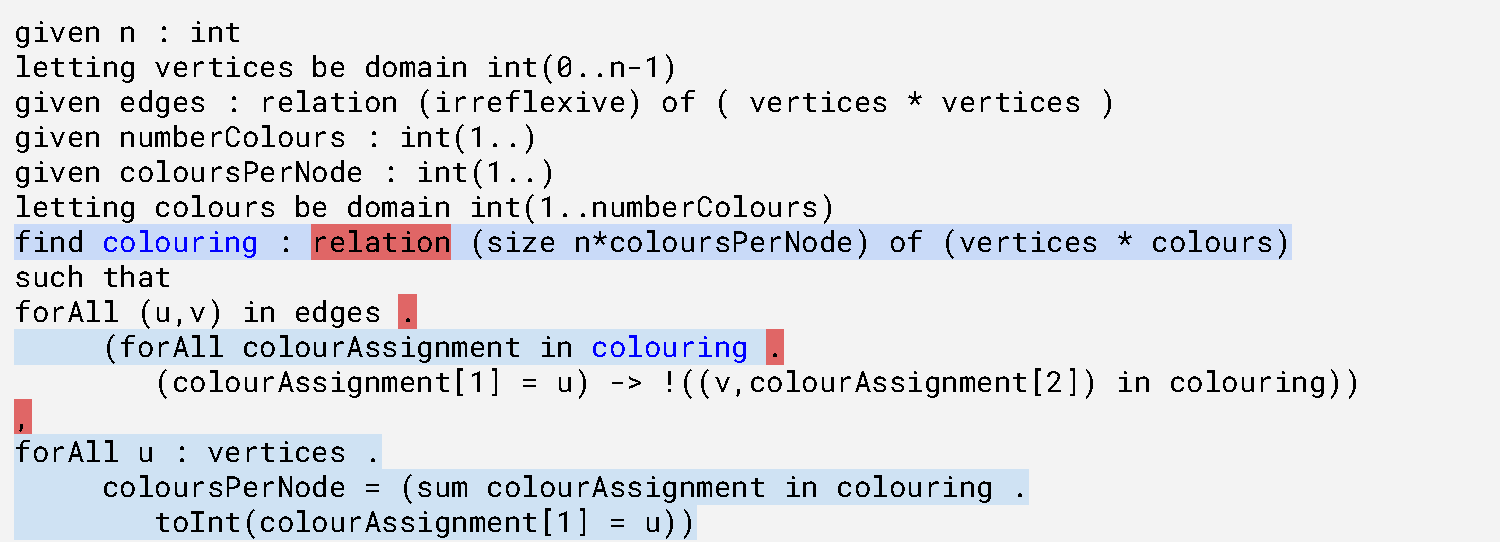
\includegraphics[width=\columnwidth]{CP2024-midrewrite.pdf}
    \caption{Parts of the specification that are interacted with during rewrite. Matched subtrees are highlighted in light blue. Names that can be used as free parameters are coloured in dark blue. Tagged nodes are highlighted in red.}
\end{figure}

\zap{
\begin{lstlisting}[caption={Matching during rewriting},label={lst:during},frame=tlrb,style=plain,classoffset=0,morekeywords={colouring},keywordstyle=\color{blue},classoffset=1,morekeywords={sum},keywordstyle=\color{red}]{Name}
given n : int
letting vertices be domain int(0..n-1)
given edges : relation (irreflexive) of ( vertices * vertices )
given numberColours : int(1..)
given coloursPerNode : int(1..)
letting colours be domain int(1..numberColours)
find colouring : relation (size n*coloursPerNode) of (vertices * colours)
such that

forAll (u,v) in edges .
     (forAll colourAssignment in colouring .
        (colourAssignment[1] = u) -> !((v,colourAssignment[2]) in colouring)),

forAll u : vertices .
     coloursPerNode = (sum colourAssignment in colouring .
        toInt(colourAssignment[1] = u))
\end{lstlisting}
}

\zap{
\noindent\texttt{\footnotesize%
given n : int\\
letting vertices be {\color{red}domain int(0..n-1)}\\
given edges : relation (irreflexive) of ( vertices * vertices )
}
}

\begin{lstlisting}[caption=Rewritten specification.,label={lst:after},frame=tlrb]{Name}
given n : int(0..100)
letting vertices be domain int(0..n-1)
given edges : relation (irreflexive) of ( vertices * vertices )
given numberColours : int(1..n)
given coloursPerNode : int(1..n)
letting colours be domain int(1..numberColours)

letting coloursSet be domain set (size coloursPerNode) of colours

find colouring : function (total) vertices --> coloursSet
such that
forAll (u,v) in edges .
     colouring(v) intersect colouring(u) = {}
\end{lstlisting}

This procedure adds an auxiliary domain of type \code{set} that will host the colours, a new decision variable of type \code{function} mapping the left-hand side of the relation to the auxiliary set, and shrinks the constraints to simply require an empty intersection of two sets. The final product can be seen in \cref{lst:after}.


\subsection{Empirical evaluation of the reformulation}

In order to test the performance of the reformulated abstract specification we have developed an instance generator that produces input parameters; this uses a simple grid search spanning a range of values for $n$ nodes and $e$ edges for the graph to be coloured, $c$ colours available and $cpn$ colours per nodes enforced.
Values. $n$: 10-40, step size 10. $e$: $n^2 *20\%-80\%$, step size 5\%. $cpn$: 2-5, step size 1. $c$: $cpn$*4-6, step size 1.

Each instance is solved using both models and the results are plotted in~\cref{fig:specs_scatter}.

Our system can also translate graphs from the Python library NetworkX into \essence relations, which allows the conversion of any of its library of graphs into instances by supplying the $c$ and $cpn$ parameters. A small selection of iconic graphs has been used for additional testing, such as obtaining the 5-fold colouring of the dodecahedral graph in~\cref{fig:coloured_graph1}.

\begin{figure}[ht]
\centering
\vspace{-10pt}
\includesvg[width=0.75\columnwidth]{dodeca_turbo_palette.svg}
  \caption{5-fold colouring of the dodecahedral graph.}
  \label{fig:coloured_graph1}
\end{figure}

\begin{figure}[ht]
\centering
  \includesvg[width=\columnwidth]{performance_scatter_plot.svg}
  \caption{Performance of the two specifications: we plot instances (with selected names listed along the horizontal axis), the reformulated specifications are green, the old specifications are blue, gold indicates both specifications time out, red indicates that the old specification times out.}
  \label{fig:specs_scatter}
\end{figure}

\section{Converting solutions to their original type}

When a reformulation changes the type of a decision variable, the solution produced by the solver will be of the transformed type. To verify that the solution of the reformulated specification is, in fact, a solution to the original problem, we must convert it back to its original type. To achieve this, we create a converter based on an \essence specification, which requires the solution of the reformulated problem as a parameter. The converter (illustrated in \cref{lst:converter}) includes all the variables declared in the original specification, along with all of its parameters. Additionally, it must have a decision variable with exactly the same name as the original specification, and a constraint mapping assignments of the new type to the old type. Solving this parameterised specification produces a solution that follows the structure of the original type that can be checked using \conjure with the \code{--validate-solution} option.

We timed the conversion of all the solutions obtained by solving the instances produced in the previous section. The worst-performing conversion took 0.56 seconds, with an overall average of 0.459 seconds. This overhead is significant only for the smallest instances.
\begin{figure}[ht]
    \centering
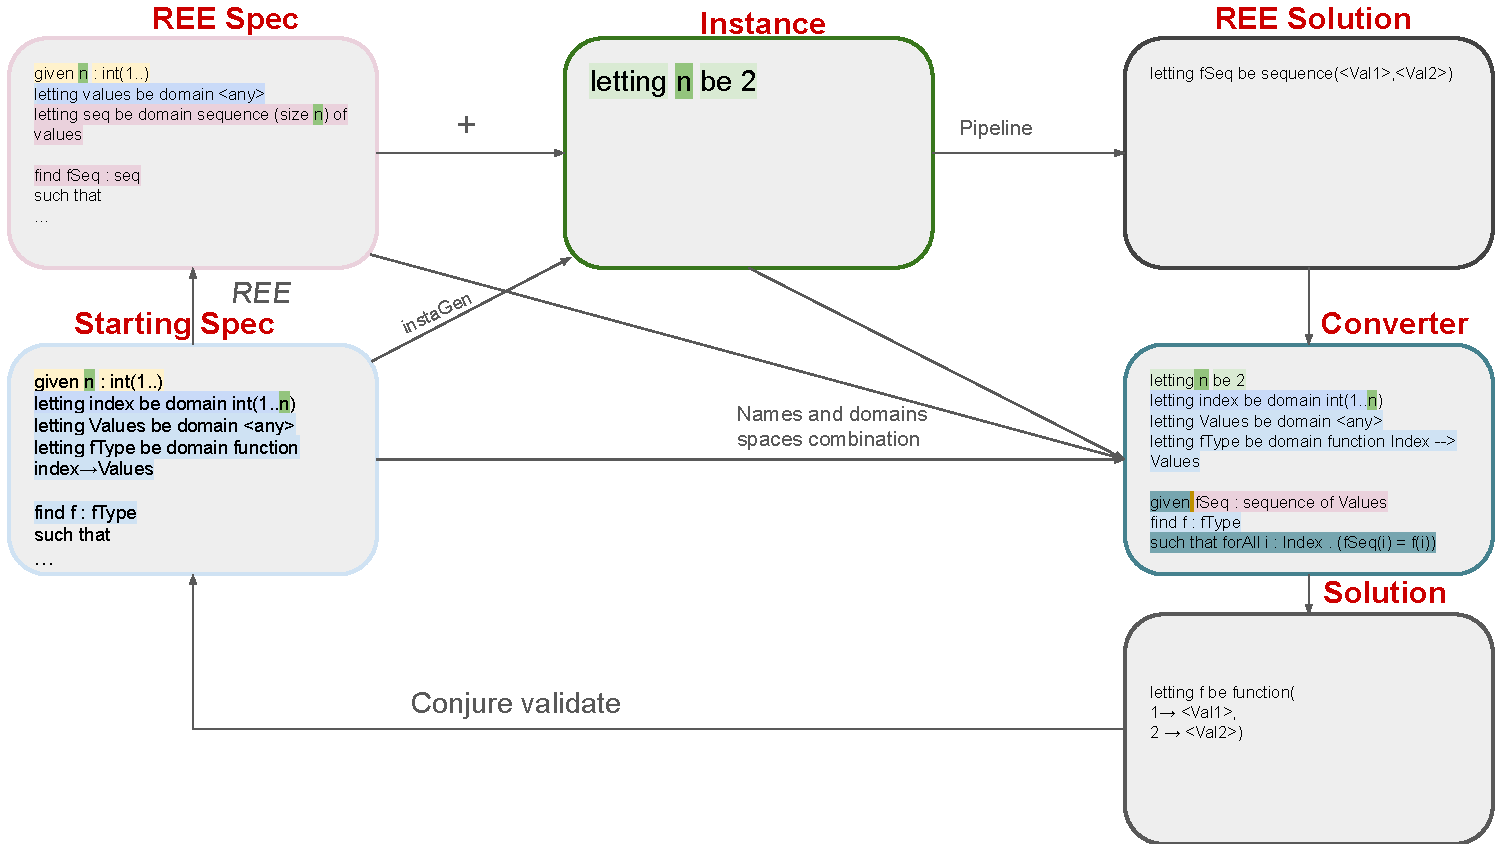
\includegraphics[width=\columnwidth]{ConverterCraft.pdf}
    \caption{Specification of the solution's converter and production flow. In this simpler example a function indexed by integers is turned into a sequence and back again.}
\end{figure}

\begin{lstlisting}[caption=Solution Converter,label={lst:converter}]{Name}
given n : int(0..100)
given numberColours, coloursPerNode : int(1..n)
letting vertices be domain int(0..n-1)
letting colours be domain int(1..numberColours)
letting coloursSet be domain set (size coloursPerNode) of colours
given solution : function (total) vertices --> coloursSet
find colouring : relation (size n*coloursPerNode) of ( vertices * colours )
such that forAll item in defined(solution) . forAll colour in solution(item) . colouring(item, colour)
\end{lstlisting}

%%%%
\zap{
Combinatorial search problems arise in many and varied settings. Consider, for example, a parcel delivery problem. Parcels and drivers must be assigned to delivery vehicles respecting capacity constraints, staff resources, shift patterns and working preferences. At the same time routes must be chosen so as to meet delivery deadlines. The problem is further complicated by the need also to optimise an objective, such as minimising fuel consumption.

Such problems are naturally characterised as a set of decision variables, each representing a choice that must be made to solve the problem at hand (such as which items are assigned to the first van leaving the depot), and a set of constraints describing allowed combinations of variable assignments (for instance, a vehicle cannot be assigned to particular route depending on its specific height or weight). A solution assigns a value to each variable satisfying all constraints. Many decision-making and optimisation formalisms take this general form, including: Constraint Programming (CP), Propositional Satisfiability (SAT), SAT Modulo Theories (SMT), and Mixed Integer Programming (MIP). Metaheuristic methods offer a complementary approach, sacrificing completeness for the ability to explore rapidly a neighbourhood of candidate solutions. These approaches have much in common, but differ in the types of decision variables and constraints they support, and the inference mechanisms used to find solutions.

In all of these formalisms the {\em model} of the problem is crucial to the efficiency with which it can be solved. A model in this sense is the set of decision variables and constraints chosen to represent a given problem. There are typically many possible models and formulating an effective model is notoriously difficult. Therefore automating modelling is a key challenge. 

This work extends our {\em Constraint Modelling Pipeline}. A user writes a problem specification in the abstract constraint specification language \essence \cite{frisch2008:essence}, capturing the structure of the problem in terms of familiar discrete mathematical objects such as sets, relations, functions, and partitions, but {\em without} committing to detailed modelling decisions. The {\sc Conjure} \cite{akgun2022conjure} automated modelling system refines an \essence specification into a solver-independent constraint model where the abstract structure is represented by a collection of primitive variables and constraints. The second stage in the pipeline, performed automatically by {\sc Savile Row} \cite{savilerow}, is in preparing the model for a particular constraint solver for one of the formalisms listed above. By following different refinement pathways the pipeline can produce a set of alternative models from a single \essence specification for evaluation or selection via machine learning. We have situated our work in the \essence language and constraint modelling pipeline because \essence allows problems to be expressed in a concise, highly structured manner. We exploit this structure to trigger the transformations we consider. 

The constraint modelling pipeline eliminates the need for specific modelling expertise in constraint programming and SAT solving.
However, the pipeline is sensitive to the way a problem is specified in \essence. This is because \conjure's refinement rules are triggered directly from the abstract variables and expressions in the \essence specification, therefore determining the reachable set of models.
This motivates our work herein: an automated reformulation system to explore the space of \essence specifications and therefore increase the size of the set of models from which we can select. Our tool uses graph formalisms throughout. An \essence specification is represented as a graph; all reformulations of an \essence specification are graph transformations. Specific properties can be preserved by transformations (such as semantic invariance), and rewrites are applied only when well-defined conditions are present. Furthermore our system uses a persistent data structure holding the history of previous reformulations, so supporting the accumulation of data for subsequent learning.
}

\section{Conclusion}

In this paper we have demonstrated an automated system for the reformulation of \essence specifications. Our system, implemented in the Graph Programs 2 language, reformulates specifications of parameterised problem classes, giving the key advantage of reformulation effort being amortised over the set of instances from the class to be solved. 
High-level \essence specifications are concise and highly structured, aiding rewriting. Furthermore, they are not tied to any particular solving paradigm, hence specification reformulations may be tested against a variety of modelling and solving choices.

{\bf Future work.}
Thanks to this foundational work, we have created the basis necessary to develop a system where the rewrite rules are produced automatically, or semi-automatically, starting from pairs of specifications that express possible reformulations. Automating the creation of rewrite rules would not only free the developer from the need to write GP2 programs but also collect rewrites from past specifications that have been refined over time in order to populate a rewriting library by distilling previous expert knowledge sitting idle in existing catalogues and literature. Another enticing future direction is the production of rewrite rules using search methods, which could be applied to any arbitrary specification. The aim would be to produce reformulations that improve the current model under consideration and are reusable.

\bibliography{main.bib}
\end{document}

\end{document}


TEMPORARY BIN 


% \essence specifications are nodes, and edges are graph transformations in a higher level graph that fully preserves the history of rewrites applied by our systems. Our tool employs a collection of cross-format translations, which are nodes in a conversion graph. This allows the search for shortest paths between formats when multiple paths are available. This approach allows the extension of the available formats to require a single converter to access all the other formats or choose time-aware paths.




\noindent\begin{minipage}{.45\textwidth}
\begin{lstlisting}[caption=Before,frame=tlrb]{Name}
given a : bool
find b : bool
find c : bool
    such that
        a = !(b /\ c)
\end{lstlisting}
\end{minipage}\hfill
\begin{minipage}{.45\textwidth}
\begin{lstlisting}[caption=After,frame=tlrb]{Name}
given a : bool
find b : bool
find c : bool
    such that
        a = (!b \/ !c)
\end{lstlisting}
\end{minipage}

a collection of software, languages and formalisms that enable a user to express a combinatorial search problem in \essence, an abstract constraint specification language, capturing its structural properties beyond the level where modelling decisions are typically made. The modelling pipeline automatically generates a model from these specifications. This eliminates the requirement for user expertise in constraint modelling while retaining the specified problem's structure intact. The system can explore alternative models and leverage properties like symmetry (add more). This is implemented by applying a type-specific refinement via conjure, which translates the specification into \essence Prime which is further refined and translated into solver-specific languages across formalisms: SMT,MIP,SMT,SAT and CP (Improve this).

Until now, refinements have been applied while lowering the model's abstraction level. With this new tool, we enable transformations that are applied to and maintain the highest level of abstraction. 

The advantages are multifold:

\begin{itemize}
    \item Rewritten models are more humanly readable.
    \item It allows the study of high level choices on the entire pipeline plus solvers in a systematic manner.
    \item It enables the synthesis of abstract specification.
    \item We can be confident of property preserving rewrites.
\end{itemize}

All our formal rewrites make use of the GP2 language and compiler. As part of its integration with our tool we developed a Python interface for it, significantly improving its usability. Among other implemented features, such as invoking GP2 programs and reading results, it is possible to apply GP2 programs to arbitrary NetworkX graphs, Python's most popular graphs library.


Rest of the paper:

\begin{itemize}
    \item Explanation of the pipeline
    \item Diagram of our system
    \item Example of a transformation being applied - step by step - (projection on the graph colouring spec, relation to function, De Morgan)
    \item Explanation of the constructed `knowledge graph' with specs, solutions and transformations that have been applied (mention persistent history of graphs)
    \item Plot or screenshot of a graph showing the exploration
\end{itemize}

\zap{
Also Known As: 

Professor Hell and his writing titled - From Graph Colouring to Constraint Satisfaction: There and Back Again
\cite{hell2006graph}

Exact Solution of Graph Coloring Problems via Constraint Programming and Column Generation  they call it 'the minimum vertex graph multicoloring problem' also the 'fractional vertex coloring', they are the optimisation versions where one has to find the 'fractional chromatic number' of a graph.

Use of fractional graph colouring for preemptive multiprocessor scheduling\cite{jansen2004preemptive}

Generalised graph colouring by a hybrid of local search and constraint programming\cite{prestwich2008generalised} 

The dodecahedron, a highly regular graph on 20 vertices, can be 7-fold coloured using 13 colours.
This takes about 10 times as long with the relational specification as with the functional one.

The functional specification finds a 2-fold colouring with 10 colours of a random graph with 40 vertices and 120 edges in about 2s, while the relational specification did not complete within 1 hour (?check).

\code{conjure solve tests/gcmulti-func.essence tests/gcmulti-40-10-2.param}

\code{1.21 real 1.94 user 0.32 sys}

\code{conjure solve tests/gcmulti.essence tests/gcmulti-40-10-2.param}

\code{Savile Row stderr: ERROR: Out of Memory}

\code{1467.39 real 1441.07 user 18.71 sys}
}
